\documentclass[12pt,compress,ngerman,utf8,t]{beamer}
\usepackage[ngerman]{babel}
\usepackage{calc}
\usepackage{ragged2e,wasysym,multicol,mathtools,tikz}
\usepackage[protrusion=true,expansion=true]{microtype}
\hypersetup{colorlinks=true}

\graphicspath{{images/}}

\title[Düstere Ecken der Logik]{Düstere Ecken der Logik}
\author[Ingo Blechschmidt]{\textcolor{white}{Ingo Blechschmidt}}
\date[2017-09-07]{\vspace*{-4em}\ \\\textcolor{white}{\scriptsize Curry Club Augsburg \\ 7. September 2017}}

%\usetheme{Warsaw}
\useinnertheme[shadow=false]{rounded}
\useoutertheme{split}
\usecolortheme{orchid}
\usecolortheme{whale}
\setbeamerfont{block title}{size={}}

\useinnertheme{rectangles}

\usecolortheme{seahorse}
\definecolor{mypurple}{RGB}{150,0,255}
\setbeamercolor{structure}{fg=mypurple}
\definecolor{myred}{RGB}{150,0,0}
\setbeamercolor*{title}{bg=myred,fg=white}
\setbeamercolor*{titlelike}{bg=myred,fg=white}

\usefonttheme{serif}
\usepackage[T1]{fontenc}
\usepackage{libertine}

\renewcommand{\_}{\mathpunct{.}\,}
\newcommand{\BB}{\mathbb{B}}
\newcommand{\M}{\mathcal{M}}
\newcommand{\R}{\mathrm{R}}
\newcommand{\NN}{\mathbb{N}}
\newcommand{\RR}{\mathbb{R}}
\newcommand{\Eff}{\mathrm{Eff}}
\newcommand{\TM}{\mathrm{TM}}
\newcommand{\STM}{\mathrm{STM}}
\newcommand{\RW}{\mathrm{RW}}
\newcommand{\lambdaC}{\lambda\mathrm{C}}
\newcommand{\PA}{\mathrm{PA}}
\newcommand{\goedel}[1]{\ulcorner #1 \urcorner}
\newcommand{\Prov}{\mathrm{Prov}}
\newcommand{\True}{\mathrm{True}}
\newcommand{\Con}{\mathrm{Con}}
\newcommand{\proves}{\vdash}
\newcommand{\defeq}{\vcentcolon=}

\newcommand{\kasten}[1]{%
  \setlength{\fboxrule}{2pt}%
  \setlength{\fboxsep}{8pt}%
  {\usebeamercolor[fg]{item}\fbox{\usebeamercolor[fg]{normal text}\parbox{0.2cm}{#1}}}}%

\newcommand{\slogan}[1]{%
  \begin{center}%
    \setlength{\fboxrule}{2pt}%
    \setlength{\fboxsep}{8pt}%
    {\usebeamercolor[fg]{item}\fbox{\usebeamercolor[fg]{normal text}\parbox{0.91\textwidth}{#1}}}%
  \end{center}%
}

\newcommand{\code}[1]{%
  \begin{center}%
    \setlength{\fboxrule}{1pt}%
    \setlength{\fboxsep}{8pt}%
    {\fbox{\parbox{0.81\textwidth}{#1}}}%
  \end{center}%
}

\setbeamertemplate{navigation symbols}{}

\setbeamertemplate{title page}[default][colsep=-1bp,rounded=false,shadow=false]
\setbeamertemplate{frametitle}[default][colsep=-2bp,rounded=false,shadow=false,center]

\newcommand{\hil}[1]{{\usebeamercolor[fg]{item}{\textbf{#1}}}}
\setbeamertemplate{frametitle}{%
  \vskip1em%
  \leavevmode%
  \begin{beamercolorbox}[dp=1ex,center]{}%
      \usebeamercolor[fg]{item}{\textbf{\textsf{\Large \insertframetitle}}}
  \end{beamercolorbox}%
}

\setbeamertemplate{footline}{%
  \leavevmode%
  \hfill%
  \begin{beamercolorbox}[ht=2.25ex,dp=1ex,right]{}%
    \usebeamerfont{date in head/foot}
    \insertframenumber\,/\,\inserttotalframenumber\hspace*{1ex}
  \end{beamercolorbox}%
  \vskip0pt%
}

\newcommand{\backupstart}{
  \newcounter{framenumberpreappendix}
  \setcounter{framenumberpreappendix}{\value{framenumber}}
}
\newcommand{\backupend}{
  \addtocounter{framenumberpreappendix}{-\value{framenumber}}
  \addtocounter{framenumber}{\value{framenumberpreappendix}}
}

\setbeameroption{show notes}

\begin{document}

% http://www.ufointernationalproject.com/wp-content/uploads/2015/11/a23.jpg
{\usebackgroundtemplate{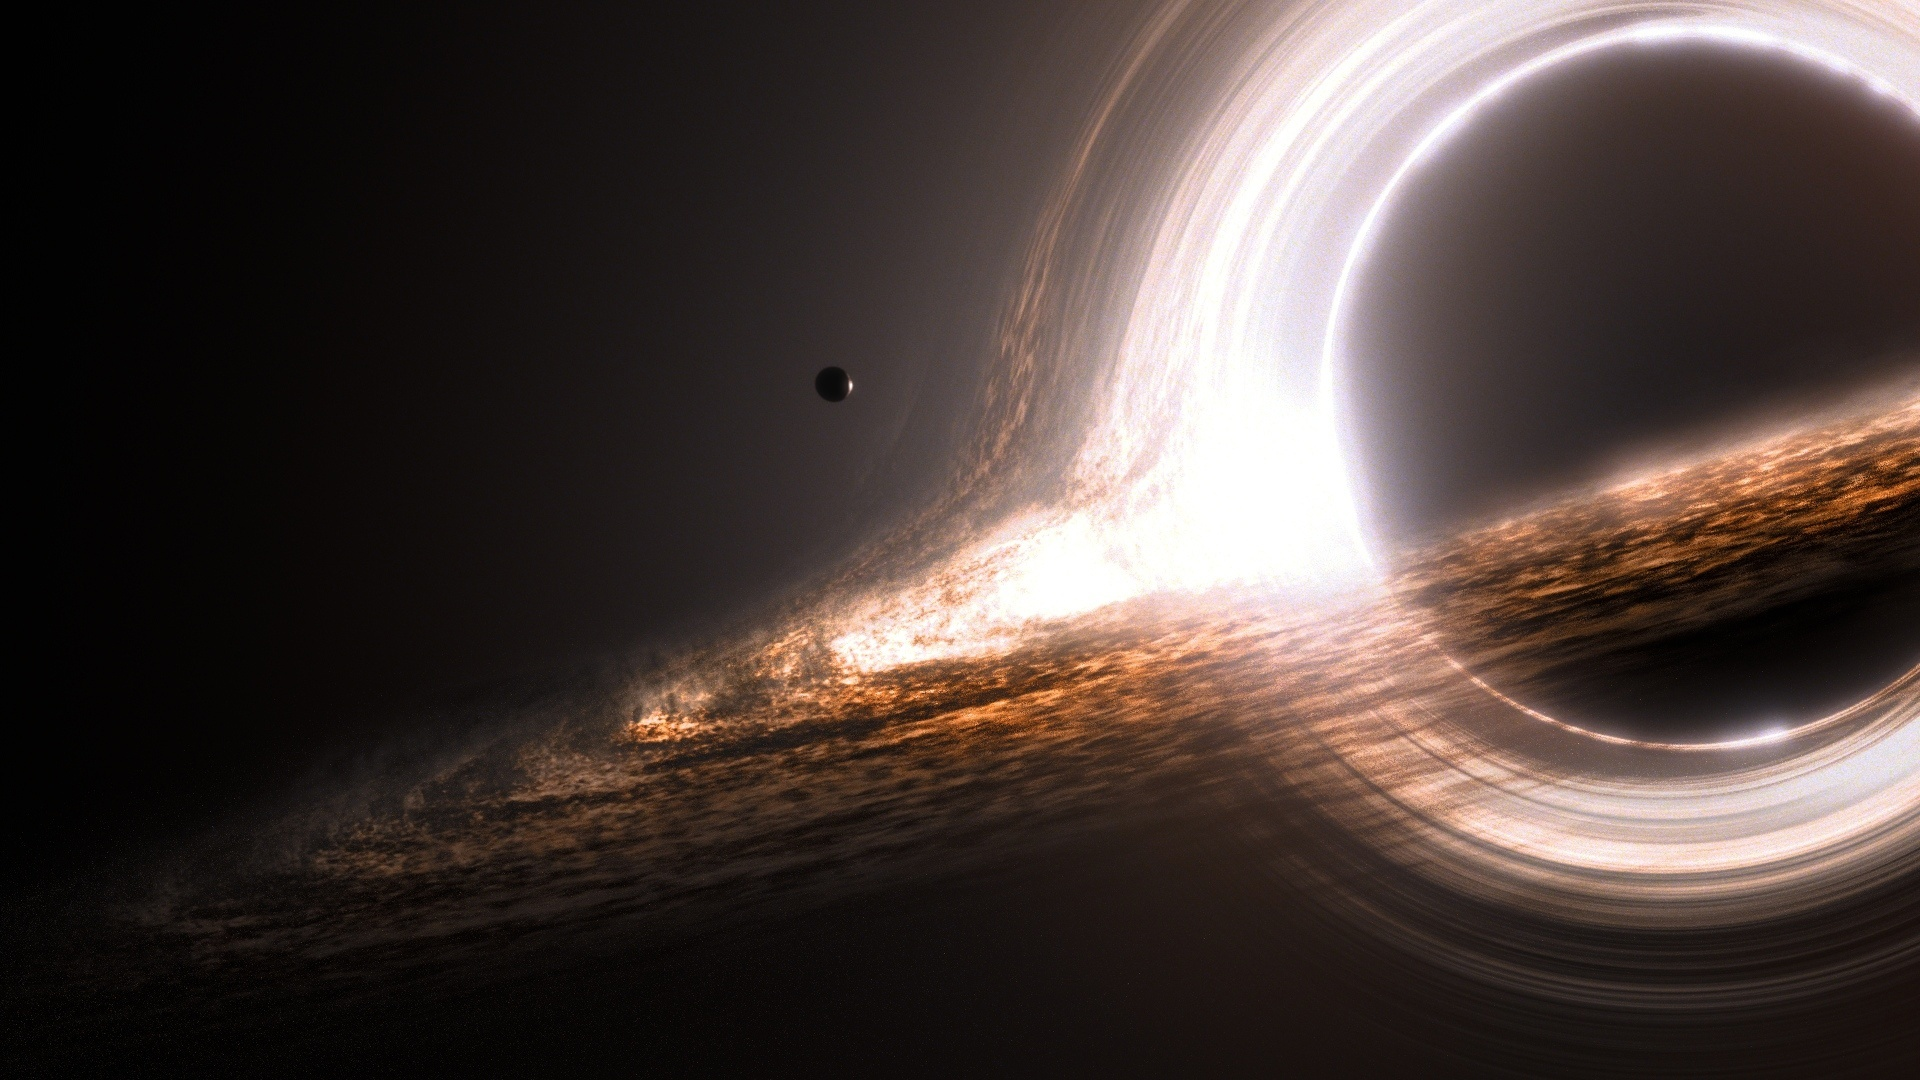
\includegraphics[height=\paperheight]{images/interstellar}}
\frame{\vspace*{12em}\titlepage}}
\frame{\tableofcontents}


\begin{frame}
  \centering
  \bigskip

  \Huge \hil{Abschnitt 0}

  \bigskip
  \Large\textbf{Der effektive Topos}
  \par
  \bigskip
  \bigskip

  \normalsize
  \raggedright

  Es gibt ein mathematisches Alternativuniversum, in dem \ldots

  \begin{enumerate}
    \item es nicht trivial ist, dass jede Zahl prim oder nicht prim ist,
    \item nicht jede Menge leer ist oder nicht leer ist,
    \item jede Funktion~$\NN \to \NN$ berechenbar ist und
    \item jede Funktion~$\RR \to \RR$ stetig ist.
  \end{enumerate}
\end{frame}

\note{
  \justifying\scriptsize
  Zu jedem Modell von Berechenbarkeit, wie etwa Turingmaschinen oder dem
  Lambda-Kalkül, gibt es eine Variante des "`effektiven Topos"'. Man kann sogar
  Maschinen der realen Welt als Grundlage verwenden; dann verlässt man die
  rigorose Mathematik, erhält aber philosophisch/phy\-si\-ka\-lisch interessante
  Aussagen.
  \medskip

  Turingmaschinen und das Lambda-Kalkül liefern zwar denselben
  Berechenbarkeitsbegriff für Funktionen~$\NN \to \NN$, sie unterscheiden sich
  aber in Fragen der Berechenbarkeit von Funktionen höherer Ordnung. Daher sind
  auch die entstehenden Topoi unterschiedlich.
  \medskip

  Mehr zum Thema:
  \begin{itemize}
    \item
    \url{https://rawgit.com/iblech/mathezirkel-kurs/master/superturingmaschinen/slides.pdf}
    \item
    \url{https://rawgit.com/iblech/mathezirkel-kurs/master/superturingmaschinen/slides-warwick2017.pdf}
  \end{itemize}
}


\section[Gödel]{Gödels Unvollständigkeitssatz}

\begin{frame}
  \centering
  \bigskip

  \Huge \hil{Abschnitt I}

  \bigskip
  \Large\textbf{Gödels Unvollständigkeitssatz}
  \par
  \bigskip

  \large

  Es gibt wahre Aussagen, die nicht beweisbar sind.

  \pause
  \bigskip
  \bigskip

  Zum Beispiel folgende:

  "`Diese Aussage ist nicht beweisbar."'
  \bigskip
  \bigskip
  \pause

  Currys Paradoxon mahnt zur Vorsicht:

  \mbox{\!\!\!\!\!\!"`Sollte diese Aussage stimmen, so ist der Mond aus Käse."'}
  \par
\end{frame}

\note{
  \justifying\scriptsize
  Wie kann es konzeptionell sein, dass es unbeweisbare wahre Aussagen gibt?
  Woher können wir von einer Aussage wissen, dass sie wahr ist, wenn nicht
  durch einen Beweis? Dieser Scheinwiderspruch wird auf den nächsten
  Folien aufgeklärt.
  \medskip

  Wie die \href{https://de.wikipedia.org/wiki/Currys_Paradoxon}{Wikipedia-} und
  \href{https://plato.stanford.edu/entries/curry-paradox/}{SEP-Artikel} zu
  Currys Paradoxon erklären, lässt sich nicht jeder grammatikalisch korrekte
  Aussagesatz menschlicher Sprache als formale Aussage im Sinne der Logik
  interpretieren.
  \medskip

  Deswegen ist die Beweisskizze von Gödels Unvollständigkeitssatz auf der
  vorherigen Folie unvollständig: Es ist korrekt, aber nicht klar, dass die
  Aussage "`Diese Aussage ist unbeweisbar"' formal verstanden werden kann.
  \medskip

  Das Problem bei Currys Paradoxon liegt übrigens nicht an der
  Selbstbezüglichkeit, sondern am Wort~"`stimmen"'.
  \par
}


\begin{frame}\frametitle{Vereinbarungen zur Metaebene}
  Auf der Metaebene wissen wir, \ldots
  \begin{enumerate}
    \item wie man mit endlichen syntaktischen Objekten operiert,

    \item was die natürlichen Zahlen sind,

    \begin{center}\begin{tikzpicture}
      \draw[-latex,dotted] (0.0,0) -- (5.5,0);
      \foreach \x in {0,1,2,3,4,5}
      \draw[shift={(\x,0)},color=black] (0pt,3pt) -- (0pt,-3pt);
      \foreach \x in {0,1,2,3,4,5}
      \draw[shift={(\x,0)},color=black] (0pt,0pt) -- (0pt,-3pt) node[below] {$\x$};
    \end{tikzpicture}\end{center}

    \item was es bedeutet, dass eine Zahl mit einer gewissen Eigenschaft
    existiert oder dass eine Behauptung für alle Zahlen stimmt.
  \end{enumerate}

  \pause

  Mögliche Wahlen der Metaebene:
  \begin{itemize}
    \item gesunder Menschenverstand mit Platonismus
    \item gesunder Menschenverstand mit Formalismus
    \item diverse formale Systeme
  \end{itemize}
\end{frame}

\note{\justifying\scriptsize
  Wenn man sich entscheidet, die Metaebene formal zu halten, verwendet man oft
  sehr schwache Systeme wie etwa
  \href{https://en.wikipedia.org/wiki/Primitive_recursive_arithmetic}{PRA}, die
  sowohl von ihren sprachlichen Mitteln als auch den erlaubten logischen
  Schlüsseln sehr eingeschränkt sind. (PRA ist so schwach, dass es noch nicht
  einmal einen Unterschied zwischen klassischem und intuitionistischem PRA
  gibt. In PRA gibt es auch keine Realisierung der aktual unendlichen Menge der
  natürlichen Zahlen.)
  \medskip

  Das macht man aus zwei Gründen: Zum einen möchte man in diesem Geschäft unter
  anderem die Konsistenz von gewissen logischen Systemen untersuchen. Um sicher
  zu gehen, dass solche Untersuchungen aussagekräftig sind, sollten sie selbst
  keine mächtigen logischen Prinzipien verwenden.
  \medskip

  Zum anderen möchte man Argumente auf der Metaebene gelegentlich auch in
  anderen Systemen internalisieren. Dazu ist es hilfreich, auf der Metaebene
  ein System zu verwenden, dass als größter gemeinsamer Nenner aller relevanten
  anderen Systeme fungieren kann. PRA ist ein solches System.
  \medskip

  Oft verwendet man aber auch starke Systeme wie Zermelo--Fraenkel-Mengenlehre mit
  Auswahlaxiom und großen Kardinalzahlaxiomen als Metaebene, um interessante
  modelltheoretische Aussagen treffen zu können.
  \par
}


\subsection[Beweisbarkeit und Wahrheit]{Beweisbarkeit und Wahrheit}

\note{\justifying\scriptsize
  Im Folgenden studieren wir \emph{Peano-Arithmetik}~($\PA$), ein wichtiges formales
  System in Logik erster Ordnung. Genauso gut könnten wir eine Formalisierung
  von Mengenlehre in Logik erster Ordnung oder diverse andere Systeme
  verwenden.
  \medskip

  Die Terme von~$\PA$ werden induktiv aus der Konstante~$0$, der
  Nachfolgeroperation~$S$ und Funktionssymbolen für jede primitiv-rekursive
  Funktion zusammengesetzt. Etwa ist~$4 \defeq S(S(S(S(0))))$ ein Term
  in~$\PA$.
  \medskip

  Aussagen in~$\PA$ werden induktiv aus folgenden Zutaten zusammengesetzt:
  \begin{itemize}
    \item $s = t$, wobei~$s$ und~$t$ beliebige Terme sind
    \item $\top$ ("`truthhood"') und~$\bot$ ("`falsehood"')
    \item $A \wedge B$, $A \vee B$, $A \rightarrow B$ und
          $\neg A$ als Abkürzung für~$A \rightarrow \bot$
    \item $\forall n\_ A(n)$ und~$\exists n\_ A(n)$
  \end{itemize}
}

\note{\justifying\scriptsize
  Die Schlussregeln und Axiome von~$\PA$ sind:
  \begin{itemize}
    \item die üblichen Schlussregeln von Logik erster Ordnung, etwa $A \wedge B
    \rightarrow A$
    \item $0$ ist kein Nachfolger: $\neg (\exists n\_ 0 = S(n))$
    \item Haben Zahlen denselben Nachfolger, so sind sie gleich: $\forall n\_
    \forall m\_ (S(n) = S(m) \rightarrow n = m)$
    \item Axiome, die die Funktionssymbole für primitiv-rekursive Funktionen
    regieren, insbesondere:
    \begin{align*}
      \forall n\_ && n + 0 &= n \\
      \forall n\_ \forall m\_ && n + S(m) &= S(n + m) \\
      \forall n\_ && n \cdot 0 &= 0 \\
      \forall n\_ \forall m\_ && n \cdot S(m) &= n \cdot m + n
    \end{align*}
    \item Für jede Aussageform~$A(n)$ je ein Induktionsaxiom:
    \[ (A(0) \wedge (\forall n\_ (A(n) \rightarrow A(n+1)))) \rightarrow
      \forall n\_ A(n). \]
  \end{itemize}
}

\begin{frame}{Beweisbarkeit und Wahrheit}
  \vspace*{-1em}
  \begin{block}{Syntaktische Qualität}
  Eine Aussage~$A$ heißt genau dann \hil{beweisbar}, wenn es in einem
  fixierten formalen System einen \hil{formalen Beweis} von~$A$ gibt:
  \vspace*{-1em}
  \[ \PA \proves A \]
  \end{block}

  \begin{block}{Semantische Qualität}
  Eine Aussage~$A$ heißt genau dann \hil{wahr}, wenn sie im
  \hil{Standardmodell} gilt:
  $\NN \models A$
  \end{block}
  
  \pause

  \begin{itemize}
    \item Jede beweisbare Aussage ist wahr.
    \item Nicht alle wahren Aussagen sind beweisbar.
    \item Es gibt \hil{Nichtstandardmodelle}:

    % https://boolesrings.org/victoriagitman/2015/04/22/an-introduction-to-nonstandard-models-of-arithmetic/
    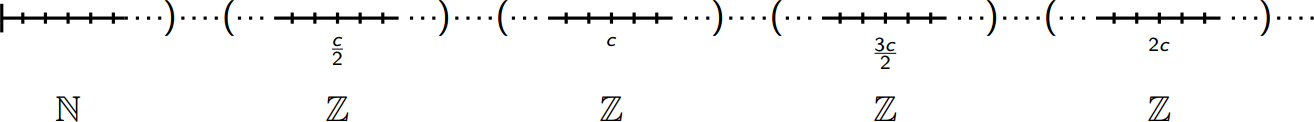
\includegraphics[scale=0.3]{nonstandard-model-of-arithmetic}

    %\item In starker Metatheorie: Alle$^\star$ konsistenten formalen Systeme
    %besitzen
  \end{itemize}
\end{frame}

\note{\justifying\scriptsize
  Die Axiome von Peano-Arithmetik sind so konzipiert, dass sie genau das Wesen
  der natürlichen Zahlen einfangen. Dieses Ziel wurde aber nicht erreicht:
  Nicht nur die üblichen natürlichen Zahlen, das Standardmodell, erfüllen die
  Peano-Axiome, auch die diversen Nichtstandardmodelle tun es.
  \medskip

  Das ist ein grundsätzliches Phänomen an Logik erster Ordnung; mit Logik
  zweiter Ordnung, bei der nicht nur über Elemente, sondern auch über
  Teilmengen quantifiziert werden kann, kann man Axiome formulieren, die nur
  von den üblichen natürlichen Zahlen und nicht von weiteren Strukturen erfüllt
  werden. Vorteile an Logik erster Ordnung sind Einfachheit und die Existenz
  von Vollständigkeitssätzen: Gilt eine Aussage in \emph{allen} Modellen, so
  ist sie beweisbar.
  \medskip

  Nur wenig Leute möchten nicht unterstellen, dass die Metaebene die
  Schlussregeln von Peano-Arithmetik mitmacht und in der~$\NN$ die Peano-Axiome
  erfüllt. Unterstellt man das, so sind beweisbare Aussagen auch wahr.
  Überdies sind beweisbare Aussagen auch in allen Nichtstandardmodellen wahr.
  \medskip

  Es wird niemals eine Haskell-Bibliothek zum Umgang mit Nichtstandardzahlen
  geben: Tennenbaum bewies 1959, dass es kein Nichtstandardmodell gibt, dessen
  Elemente man als Bitfolgen kodieren könnte, sodass Addition oder
  Multiplikation berechenbar sind.
  \medskip

  Mehr zu Nichtstandardmodellen steht auf dem
  \href{https://boolesrings.org/victoriagitman/2015/04/22/an-introduction-to-nonstandard-models-of-arithmetic/}{Blog von Victoria Gitman}.
  \par
}

\note{\justifying\scriptsize
  Sei~$A$ etwa die formale Aussage~$\forall n\_ \forall m\_ (n+m)^2 = n^2 + 2nm
  + m^2$. Dann bedeutet~$\NN \models A$, dass für alle gewöhnlichen Zahlen die
  binomische Formel gilt. Ist~$M$ irgendein Nichtstandardmodell, so bedeutet~$M
  \models A$, dass für alle Zahlen des Nichtstandardmodells die binomische
  Formel gilt. (Die Aussage~$A$ ist übrigens beweisbar und daher in allen
  Modellen gültig.)
  \medskip

  Die meisten Leute erachten~$\PA$ als \emph{konsistent}, d.\,h. die
  Aussage~$\bot$ (oder äquivalent die Aussage~$0 = 1$) als nicht
  beweisbar. Denn wenn~$0 = 1$ beweisbar wäre, so wäre auch~$0 = 1$ im
  Standardmodell~$\NN$ (wenn man akzeptiert, dass~$\NN$ die Peano-Axiome
  erfüllt); dem ist aber nicht so.
  \medskip

  Ein rein syntaktischer und finitistisch zulässiger Beweis der Konsistenz
  von~$\PA$ wurde aber noch nicht erbracht. Es macht Spaß, die Inkonsistenz
  von~$\PA$ in Betracht zu ziehen; sie ist aber extrem unwahrscheinlich.
  \par
}


\subsection{Quines}

\begin{frame}{Quines}
  Wir schreiben~$\goedel{A}$ für die \hil{Gödelnummer} einer Aussage~$A$.

  \begin{block}{Reflektion von Beweisbarkeit}
    Es gibt eine Aussageform~$\Prov(n)$, sodass für jede Aussage~$A$
    genau dann~$\Prov(\goedel{A})$ wahr ist, wenn~$A$ beweisbar ist:
    \vspace*{-0.8em}
    \[ \NN \models \Prov(\goedel{A}) \quad\text{genau dann, wenn}\quad
      \PA \proves A. \]
  \end{block}
  \pause

  Mit dem \hil{Diagonallemma} gibt es eine Aussage~$G$ mit
  \vspace*{-0.2em}
  \[ \PA \proves (G \leftrightarrow \neg (\Prov(\goedel{G}))). \]
  \vspace*{-1em}
  \pause
  \justifying
  \begin{enumerate}
  \item Angenommen $\PA \proves G$.
  Dann $\PA \proves \neg (\Prov(\goedel{G}))$,
  also~$\NN \models \neg (\Prov(\goedel{G}))$,
  also nicht~$\NN \models \Prov(\goedel{G})$,
  also ist~$G$ nicht beweisbar,
  also folgt ein Widerspruch.
  \item Also ist~$G$ nicht beweisbar,
  somit~$\NN \models \neg\Prov(\goedel{G})$.
  \item Also~$\NN \models G$, d.\,h.~$G$ ist wahr.
  \end{enumerate}
\end{frame}

\note{\justifying\scriptsize
  Die mit dem Diagonallemma konstruierte Aussage~$G$ drückt umgangssprachlich
  aus: "`Aussage~$G$ ist nicht beweisbar."' Der auf der vorhergehenden Folie
  gegebene Beweis von Gödels Unvollständigkeitssatz ist also eine
  Ausformalisierung der anfangs gegebenen Beweisskizze. Das Diagonallemma
  ermöglicht, Selbstbezüglichkeit zu elimieren.
  \medskip

  Dieser (Meta-)Beweis von Gödels Unvollständigkeitssatz liefert ein explizites
  Beispiel für eine Aussage, die im Standardmodell wahr ist, aber keinen
  formalen Beweis in~$\PA$ besitzt. Die so erhaltene Aussage wurde aber
  speziell für diese Argumentation konstruiert. Es gibt viele weitere Beispiele
  für unbeweisbare wahre Aussagen, die inhaltlich viel interessanter sind und
  auf den ersten Blick keinerlei Verbindungen zur mathematischen Logik
  aufzuweisen scheinen, insbesondere nicht Selbstbezüglichkeit oder Begriffe
  wie~"`Beweisbarkeit"' enthalten.
  \medskip

  Das Argument auf der vorhergehenden Folie für~$\PA \not\proves G$, war
  semantisch: Es verwendete, dass~$\NN$ ein Modell von~$\PA$ ist. Ein rein
  syntaktischer Beweis, der nur die Annahme der Konsistenz von~$\PA$ verwendet,
  ist auch möglich: Angenommen, es gibt einen formalen Beweis von~$G$. Dieser
  hat eine Gödelnummer, sodass man ihn in das formale System bringen kann: Es
  folgt~$\PA \proves \Prov(\goedel{G})$. Zugleich gilt~$\PA \proves
  \neg(\Prov(\goedel{G}))$. Also~$\PA \proves \bot$. Widerspruch.
  \medskip

  Die Negation von~$G$ ist in $\PA$ ebenfalls nicht beweisbar: Wenn doch, wäre
  sie wahr, ist sie aber nicht. Ein syntaktischer Beweis ist nicht bekannt,
  aber \emph{Rossers Trick} liefert eine leichte Variante~$G'$, von der
  syntaktisch~$\PA \not\proves G'$ und~$\PA \not\proves \neg G'$ nachweisbar
  sind (nur unter der Konsistenzannahme).
  \par
}

\note{\justifying\scriptsize
  Die Aussage~$G$, die das Diagonallemma liefert, lautet ins Deutsche übersetzt wie
  folgt:
  \medskip

  "`Die Aussage, die man erhält, wenn man in der Aussage \glq Die Aussage, die man
  erhält, wenn man in der Aussage~$x$ die vorkommende Variable durch die
  Gödelnummer dieser Aussage ersetzt, ist nicht beweisbar.\grq{} die
  vorkommende Variable durch die Gödelnummer dieser Aussage ersetzt, ist nicht
  beweisbar."'
  \par
}

\begin{frame}{Goodsteinsche Folgen}
  \vspace*{-0.5em}
  Beginne etwa mit~$35$. Schreibe die Zahl in
  \hil{hereditary base $\boldsymbol{2}$}:
  \begin{align*}
    35 &= 1 \cdot 2^5 + 1 \cdot 2^1 + 1 \cdot 2^0 \\
       &= 1 \cdot 2^{1 \cdot 2^2 + 1 \cdot 2^0} + 1 \cdot 2^1 + 1 \cdot 2^0. \\
  \intertext{Ersetze alle Vorkommen von~$2$ durch~$3$:}
       &\mathrel{\phantom{=}} 1 \cdot 3^{1 \cdot 3^3 + 1 \cdot 3^0} + 1 \cdot 3^1 + 1 \cdot 3^0 \\
       &= 1 \cdot 3^{28} + 3 + 1 \\
       &= 22876792454965.
  \intertext{Ziehe dann~$1$ ab:}
       &\mathrel{\phantom{=}} 22876792454964.
  \end{align*}
  Mach immer so weiter.
  \pause

  \begin{itemize}
    \item Schlussendlich ist das Ergebnis~$0$.
    \item $\PA$ kann nicht beweisen, dass dem immer so ist.
  \end{itemize}
\end{frame}


\subsection[Undefinierbarkeit]{Undefinierbarkeit von Wahrheit}

\begin{frame}{Undefinierbarkeit von Wahrheit}
  \begin{block}{Reflektion von Beweisbarkeit}
    Es gibt eine Aussageform~$\Prov(n)$, sodass für jede Aussage~$A$
    genau dann~$\Prov(\goedel{A})$ wahr ist, wenn~$A$ beweisbar ist:
    \vspace*{-0.8em}
    \[ \NN \models \Prov(\goedel{A}) \quad\text{genau dann, wenn}\quad
      \PA \proves A. \]
  \end{block}

  Kann man auch Wahrheit reflektieren? Gibt es eine Aussageform~$\True(n)$,
  sodass für jede Aussage~$A$ genau dann~$\True(\goedel{A})$ wahr ist, wenn~$A$
  wahr ist?
    \[ \NN \models \True(\goedel{A}) \quad\text{genau dann, wenn}\quad
      \NN \models A \]
  \pause
  \vspace*{-1em}

  \hil{Nein:} Mit dem Diagonallemma gäbe es eine Aussage~$A$ mit
  \[ \PA \models (A \leftrightarrow \neg(\True(\goedel{A}))). \]
  Zu deutsch besagte~$A$: "`Aussage~$A$ ist nicht wahr."'
  Diese Aussage wäre genau dann wahr, wenn sie nicht wahr ist.
\end{frame}


\subsection[Konsistenz]{Konsistenzreflektion}

\begin{frame}{Konsistenzreflektion}
  Sei wie vorher~$G$ die Aussage~"`Aussage~$G$ ist nicht beweisbar"'.
% \[ \PA \proves (G \leftrightarrow \neg (\Prov(\goedel{G}))). \]

  Wir wissen: Ist~$\PA$ konsistent (d.\,h. ist~$1 = 0$ nicht beweisbar),
  so stimmt~$G$.
  \bigskip
  \pause

  Das dafür präsentierte Argument könnten wir formalisieren. Daher folgt:
  \[ \PA \proves (\neg(\Prov(\goedel{1 = 0})) \rightarrow G). \]
  \pause\justifying
  Ist~$\PA$ konsistent, so folgt:
  \begin{center}\hil{$\boldsymbol{\PA}$ kann die Konsistenz
  von~$\boldsymbol{\PA}$ nicht beweisen.}\end{center}
  Denn aus~$\PA \proves \neg(\Prov(\goedel{1 = 0}))$
  folgte $\PA \proves G$, was unter der Konsistenzannahme
  falsch ist.
  \par
\end{frame}

\begin{frame}{Going deeper}
  Wir schreiben~"`$\Con$"' für~"`$\neg(\Prov(\goedel{1=0}))$"'.
  \bigskip

  Wir wissen: Genau dann ist~$\PA$ konsistent, wenn~$\PA$ die Konsistenz
  von~$\PA$ nicht beweisen kann.
  \bigskip

  Das dafür präsentierte Argument könnten wir formalisieren. Daher folgt:
  \[ \PA \proves (\Con \leftrightarrow \neg(\Prov(\Con))). \]
\end{frame}


\section[Halteproblem]{Das Halteproblem}

\begin{frame}
  \centering
  \bigskip

  \Huge \hil{Abschnitt II}

  \bigskip
  \Large\textbf{Spiel und Spaß mit \\ Berechenbarkeitstheorie}
  \par
  \bigskip
  \bigskip

  \centering
  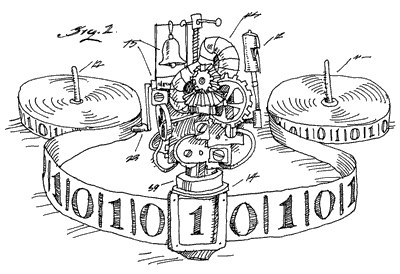
\includegraphics[scale=0.4]{turing-machine}
  \par
\end{frame}


\subsection[Unentscheidbarkeit]{Unentscheidbarkeit des Halteproblems}

\begin{frame}{Unentscheidbarkeit des Halteproblems}
  Ein \hil{Halteorakel} ist ein Programm, dass ein Programm~$P$ als Eingabe liest
  und korrekt ausgibt: "`$P$ hält"' oder~"`$P$ hält nicht"'.
  \bigskip
  \pause

  Wenn es ein Halteorakel gäbe, könnte man auch folgendes Programm~$Q$
  entwickeln:
  \code{
    Befrage das Halteorakel, ob Programm~$Q$ hält.

    Falls ja: Gehe in eine Endlosschleife.

    Falls nein: Halte.
  }
  \pause
  Das Programm~$Q$ hält genau dann, wenn es nicht hält.
  \bigskip

  Ein Halteorakel gibt es nicht.
\end{frame}

\note{\justifying\scriptsize
  Ein praktisch verwendbares Halteorakel wäre extrem nützlich, da man mit ihm
  auf einen Schlag unzählige offene mathematische Vermutungen klären könnte.
  Etwa ist momentan noch unbekannt, ob es ungerade perfekte Zahlen gibt. Hätte
  man ein Halteorakel, könnte man diese Frage sofort klären, indem man es
  befragt, ob ein Programm, dass alle ungeraden natürlichen Zahlen abläuft und
  genau dann abbricht, wenn es eine perfekte Zahl gefunden hat, hält.
  \par
}

\begin{frame}{Chaitinsche Haltewahrscheinlichkeit}
  Sei~$\Omega$ die Zahl
  \[ \Omega = \sum_p 2^{-|p|} = 2^{-c_0} + 2^{-c_1} + 2^{-c_2} + 2^{-c_3} + \cdots\!, \]
  wobei~$c_n$ die Anzahl derjenigen Programme der Länge~$n$ ist, welche halten.

  \begin{itemize}
    \item $\Omega$ ist eine wohldefinierte Zahl zwischen~$0$ und~$1$.
    \item Sind die ersten~$N$ Nachkommaziffern von~$\Omega$ bekannt,
    so lässt sich das Halteproblem für alle Programme der Länge~$\leq N$ lösen.
    \pause
    \item $\Omega$ ist nicht berechenbar.
    \pause
    \item Es gibt eine konkrete Zahl~$N$, sodass~$\PA$ keine Vermutung über
    mehr als~$N$ Nachkommaziffern beweisen kann.
  \end{itemize}
\end{frame}

\note{\justifying\scriptsize
  Der amerikanische Physiker und Informatiker Charles Bennet~(*~1943) und der
  berühmte Wissenschaftsjournalist Martin Gardner~(*~1914, †~2010) schrieben
  Folgendes über~$\Omega$:
  \medskip

  "`Die Konstante~$\Omega$ verkörpert eine enorme Menge an Wissen auf sehr kleinem Raum.
  Die ersten paar Tausend Ziffern, die problemlos auf einem kleinen Stück Papier
  Platz finden könnten, enthalten die Antworten auf mehr mathematische Fragen,
  als man im ganzen Universum aufschreiben könnte.
  \medskip

  Im Laufe der Menschheitsgeschichte strebten Mystiker und Philosophen stets nach einem
  kompakten Schlüssel zu universeller Weisheit, einer endlichen Formel
  oder einem Text, der, wenn bekannt und verstanden, Antworten auf alle Fragen
  liefern würde; man denke nur an die Versuche, der Bibel, dem Koran oder dem I~Ging
  Weissagungen zu entlocken [\ldots].
  \medskip

  Solche Quellen universeller Weisheit sind herkömmlicherweise vor beiläufigem
  Zugriff ge\-schützt: indem sie schwer zu finden, wenn gefunden schwierig zu
  verstehen und gefährlich zu benutzen sind, dazu neigend, mehr und
  tiefere Fragen zu beantworten als sich der Suchende wünschte. Das esoterische
  Buch ist, wie Gott, einfach und dennoch unbeschreibbar. Es ist allwissend, und
  verändert alle, die es kennen.
  \medskip

  $\Omega$ ist in vielerlei Hinsicht eine kabbalistische Zahl. Dem menschlichen
  Verstand ist sie bekannt, aber unkennbar. Um sie im Detail zu erfahren, müsste
  man ihre unberechenbare Ziffernfolge als Glaubensgrundsatz einfach hinnehmen,
  genau wie die Worte eines heiligen Texts."'
  \par
}


\subsection[Unabhängigkeit]{Unabhängigkeit}

\begin{frame}{Ein Programm mit unbeweisbarem Halteverhalten}
  Wir betrachten folgendes Programm~$P$:
  \code{
    Laufe systematisch alle formalen Beweise ab.
    Sobald ein Beweis von~$1 = 0$ gefunden wurde, halte.
  }
  \pause

  \begin{itemize}
    \item Das Programm~$P$ hält nicht.
    \item Die Aussage, dass~$P$ nicht halte, ist in~$\PA$ nicht beweisbar.
    \pause
    \item Sei~$n$ die Anzahl Zustände, die eine Umsetzung von~$P$ als
    Turingmaschine benötigt. Dann entzieht sich jede Vermutung
    über~$\mathrm{BB}(n)$ der Beweisbarkeit in~$\PA$.
  \end{itemize}
\end{frame}


\subsection{Das universelle Programm}

\begin{frame}{Das universelle Programm}
  Wir betrachten folgendes Programm~$P$:
  \code{
    Laufe systematisch alle formalen Beweise ab.
    Sobald ein Beweis einer Aussage der Form
    "`Die Ausgabe von Programm~$P$ ist nicht die Liste
    $x_1,\ldots,x_n$"'
    gefunden wurde, gib die Liste~$x_1,\ldots,x_n$ aus und halte.
  }

  \begin{enumerate}
    \item $\PA$ beweist, dass~$P$ eine endliche Liste von Zahlen ausgibt.
    \item\justifying Für jede endliche Liste von Zahlen gibt es ein
    Universum~$M$, sodass~$P$ genau diese Liste ausgibt, wenn man es in~$M$
    ausführt.
  \end{enumerate}
\end{frame}

\note{\justifying\scriptsize
  In~$\NN$ ausgeführt, wird~$P$ nie halten.
  \medskip

  In geeigneten Nichtstandardmodellen dagegen wird~$P$ nach einer
  Nichtstandardzahl von Schritten halten.
  \medskip

  Mehr dazu steht auf dem
  \href{http://jdh.hamkins.org/the-universal-algorithm-a-new-simple-proof-of-woodins-theorem/}{Blog
  der MathOverflow-Legende und Mengentheoretikers Joel David Hamkins}.
  \par
}


\section[Zufall]{Randomisierte Strategien}

\begin{frame}
  \centering
  \bigskip

  \Huge \hil{Abschnitt III}

  \bigskip
  \Large\textbf{Zufall als wertvolle Ressource}
  \par
  \normalsize
  \raggedright
  \bigskip

  \begin{center}
    \kasten{} \qquad \kasten{}
  \end{center}

  \pause
  \bigskip
  \justifying

  Alice versteckt zwei verschiedene reelle Zahlen in Boxen.
  Bob darf in eine der Boxen hineinschauen und dann einen Tipp abgeben,
  welche der Zahlen größer sei.
  \bigskip

  \justifying
  Es gibt eine \hil{randomisierte Strategie}, mit der Bobs
  Gewinnwahrscheinlichkeit bei jeder Wahl
  von~$x$ und~$y$ mehr als~$50\,\%$ beträgt.
 \bigskip
  \pause

  \begin{center}\begin{tikzpicture}
    \draw (-3.0,0) -- (3.0,0);
    \foreach \x in {-2,0.5,2}
      \draw[shift={(\x,0)},color=black] (0pt,3pt) -- (0pt,-3pt);
    \draw[shift={(-2,-0.4)},color=black] node {$x$};
    \draw[shift={(0.5,-0.4)},color=black] node {$r$};
    \draw[shift={(2,-0.4)},color=black] node {$y$};
  \end{tikzpicture}\end{center}
\end{frame}


\end{document}
